%
% File acl2016.tex
%
%% Based on the style files for ACL-2015, with some improvements
%%  taken from the NAACL-2016 style
%% Based on the style files for ACL-2014, which were, in turn,
%% Based on the style files for ACL-2013, which were, in turn,
%% Based on the style files for ACL-2012, which were, in turn,
%% based on the style files for ACL-2011, which were, in turn,
%% based on the style files for ACL-2010, which were, in turn,
%% based on the style files for ACL-IJCNLP-2009, which were, in turn,
%% based on the style files for EACL-2009 and IJCNLP-2008...

%% Based on the style files for EACL 2006 by
%%e.agirre@ehu.es or Sergi.Balari@uab.es
%% and that of ACL 08 by Joakim Nivre and Noah Smith

\documentclass[12pt]{article}
\usepackage{acl2016}
\usepackage{times}
\usepackage{url}
% \usepackage{ctex}
\usepackage{amsmath,amscd,amsbsy,amssymb,latexsym,url,bm,amsthm}
\usepackage{amsmath}
\usepackage{amssymb}
\usepackage{graphicx}
\usepackage{hyperref}
\usepackage{listings}
\usepackage{float}
\lstset{
basicstyle=\footnotesize\ttfamily,
breaklines=true,
}

\usepackage{listings}
\usepackage{color}

\aclfinalcopy

% \definecolor{mygreen}{rgb}{0,0.6,0}
% \definecolor{mygray}{rgb}{0.5,0.5,0.5}
% smaller than 5cm (the original size); we will check this
% in the camera-ready version and ask you to change it back.

\newcommand\BibTeX{B{\sc ib}\TeX}

\title{SE305 COURSE PROJECT FINAL REPORT}

\author{Jeremy Liu, Qianyang Peng, Jingyu Cui}
\date{11/28/2016}
% Useful Command:
% \url{acl2016.org/index.php?article_id=9}
% {\small\verb|***|}
% {\small\tt acl2016.pdf}
% wew\ref{sec:abs}

% \begin{quote}
% \begin{verbatim}
% \usepackage{times}
% \usepackage{latexsym}
% \end{verbatim}
% \end{quote}

% \begin{table}[h]
% \begin{center}
% \begin{tabular}{|l|rl|}
% \hline \bf Type of Text & \bf Font Size & \bf Style \\ \hline
% paper title & 15 pt & bold \\
% author names & 12 pt & bold \\
% \hline
% \end{tabular}
% \end{center}
% \caption{\label{font-table} Font guide. }
% \end{table}

% footnote here\footnote{This is how a footnote should appear.}


% \begin{table}
% \centering
% \small
% \begin{tabular}{cc}
% \begin{tabular}{|l|l|}
% \hline
% {\bf Command} & {\bf Output}\\\hline
% \verb|{\"a}| & {\"a} \\
% \verb|{\^e}| & {\^e} \\
% \verb|{\aa}| & {\aa}  \\\hline
% \end{tabular} &
% \begin{tabular}{|l|l|}
% \hline
% {\bf Command} & {\bf  Output}\\\hline
% \verb|{\c c}| & {\c c} \\
% \verb|{\l}| & {\l} \\
% \verb|{\ss}| & {\ss} \\\hline
% \end{tabular}
% \end{tabular}
% \caption{Example commands for accented characters, to be used in, e.g., \BibTeX\ names.}\label{tab:accents}
% \end{table}

% \label{sec:intro}
% wew\ref{sec:intro}

% \begin{figure}[!htp]
% \centering
% \includegraphics[width=0.5\linewidth]{Top20.png}
% \caption{Top-20 words from class "appearance"}
% \end{figure}


% \begin{quote}
% ``Gusfield \shortcite{Gusfield:97,Aho:72} \cite{APA:83}   showed that ...''
% \end{quote}
\begin{document}
\maketitle
\tableofcontents
\newpage
\pagenumbering{arabic}


\section{Model Design}

Our models were designed with Workbench. The diagrams are much like ER diagrams but the relationships between entities are implicit. Besides the basic requirements, our design provides advanced functions including:
\begin{enumerate}
	\item We store the label of entities and text of descriptions in \textbf{all languages}, not only in English.
	\item For claims, we store the \textbf{qualifiers} in addition to the mainsnaks.
	\item For all the snaks and qualifiers, we designed tables to store various types of \textbf{datavalues}.
\end{enumerate}

Our design contains nine tables and satisfies BCNF. Moreover, we used \emph{utf8mb4} dataset to support different language characters.

The ER Diagram can be found in Figure 1. Details of the design are included in the next section.

The programming tools we used:
\begin{enumerate}
	\item Table design and create schema: MySQL Workbench
	\item File parsing and data insert: Python3
	\item User interface: Apache \& PHP
\end{enumerate}
\begin{figure*}
\label{ER DIAGRAM}
\centering
\includegraphics[width=0.8\linewidth]{ER.png}
\caption{The ER diagram of our design}
\end{figure*}
\section{Table Designs}
We finished our table design according to our model design. Our final design contains 9 tables. Reference and aliases are not stored in our tables, while all other information in different languages are stored. The design of our tables is elaborated below:
\subsection{entity}
Table schema:
\lstset{language=SQL}
\begin{lstlisting}
CREATE TABLE IF NOT EXISTS `wikidata`.`entity` (
  `serial_id` BIGINT(32) NOT NULL AUTO_INCREMENT,
  `entity_id` VARCHAR(32) NOT NULL,
  `entity_language` VARCHAR(16) NOT NULL,
  `entity_type` VARCHAR(16) NULL DEFAULT NULL,
  `entity_text` VARCHAR(255) NULL DEFAULT NULL,
  PRIMARY KEY (`serial_id`),
  INDEX `EID` (`entity_id` ASC),
  INDEX `ELANG` (`entity_language` ASC),
  INDEX `ETYPE` (`entity_type` ASC),
  INDEX `ETEXT` (`entity_text` ASC))
ENGINE = InnoDB
\end{lstlisting}
The data stored in corresponding fields:
\begin{itemize}
\item \textbf{serial\_id}: Auto incremental serial ID. Since language information is introduced here and entity ID cannot be used as a Primary Key, we use this serial\_id here as a Primary Key.
\item \textbf{entity\_id}: ID of the corresponding entity. Eg. Q5, P110, Q123423, etc.
\item \textbf{entity\_language}: Language of the label of the corresponding entity. Eg. Zh-cn, en, etc.
\item \textbf{entity\_type}: The entity type identifier. "item" for data items, and "property" for properties.
\item \textbf{entity\_text}: Contains the labels in different languages. Eg. square kilometre, Kilometro quadrato, Vierkante kilometer, etc.
\end{itemize}
Indexed tables: besides indexing the Primary Key serial\_id, other keys including entity\_id, entity\_language and entity\_type are also indexed.
\subsection{description}
\lstset{language=SQL}
Table schema:
\begin{lstlisting}
CREATE TABLE IF NOT EXISTS `wikidata`.`description` (
  `serial_id` BIGINT(32) NOT NULL AUTO_INCREMENT,
  `entity_id` VARCHAR(32) NOT NULL,
  `desc_language` VARCHAR(8) NULL,
  `desc_text` VARCHAR(255) NULL,
  PRIMARY KEY (`serial_id`),
  INDEX `EID` (`entity_id` ASC),
  INDEX `DLANG` (`desc_language` ASC))
ENGINE = InnoDB
\end{lstlisting}
The data strored in corresponding fields:
\begin{itemize}
\item \textbf{serial\_id}: Same as in table 'entity'.
\item \textbf{entity\_id}: Same as in table 'entity'.
\item \textbf{desc\_language}: Similar to entity\_language in table 'entity'.
\item \textbf{desc\_text}: Similar to entity\_text in table 'entity'.
\end{itemize}
Indexed tables: besides indexing the Primary Key serial\_id, other keys including entity\_id, desc\_language and are also indexed.
\subsection{mainsnak}
\lstset{language=SQL}
Table schema:
\begin{lstlisting}
CREATE TABLE IF NOT EXISTS `wikidata`.`mainsnak` (
  `snak_id` VARCHAR(64) NOT NULL,
  `entity_id` VARCHAR(32) NOT NULL,
  `property_id` VARCHAR(32) NOT NULL,
  `serial` INT(4) NOT NULL,
  `claimtype` VARCHAR(32) NULL DEFAULT NULL,
  `snaktype` VARCHAR(32) NULL DEFAULT NULL,
  `datatype` VARCHAR(32) NULL DEFAULT NULL,
  `rank` VARCHAR(32) NULL DEFAULT NULL,
  PRIMARY KEY (`snak_id`),
  INDEX `EID` (`entity_id` ASC),
  INDEX `PID` (`property_id` ASC),
  INDEX `CTYPE` (`claimtype` ASC),
  INDEX `STYPE` (`snaktype` ASC),
  INDEX `DTYPE` (`datatype` ASC))
ENGINE = InnoDB
\end{lstlisting}
The data stored in corresponding fields:
\begin{itemize}
\item \textbf{snak\_id}: An arbitrary identifier for the claim, used as Primary Key of this table.
\item \textbf{entity\_id}: ID of the entity this claim belongs to.
\item \textbf{property\_id}: The property this claim is describing.
\item \textbf{serial}: This field is X means this is the Xth claim of this property.
\item \textbf{claimtype}: The type of the claim - currently either statement or claim.
\item \textbf{snaktype}: The type of the snak. Currently, this is one of value, somevalue or novalue.
\item \textbf{datatype}: The datatype field indicates how the value of the Snak can be interpreted. This fields indicate the concrete table begining with "datavalue\_"
\item \textbf{rank}: The rank expresses whether this value will be used in queries, and shown be visible per default on a client system. The value is either preferred, normal, or deprecated.
\end{itemize}
\subsection{datavalue\_string}
\lstset{language=SQL}
Table schema:
\begin{lstlisting}
CREATE TABLE IF NOT EXISTS `wikidata`.`datavalue_string` (
  `snak_id` VARCHAR(64) NOT NULL,
  `value` VARCHAR(255) NULL DEFAULT NULL,
  PRIMARY KEY (`snak_id`))
ENGINE = InnoDB
\end{lstlisting}
The data strored in corresponding fields:
\begin{itemize}
\item \textbf{snak\_id}: Primary key. Refering to the table mainsnak.
\item \textbf{value}: The content of the string.
\end{itemize}
\subsection{datavalue\_time}
\lstset{language=SQL}
Table schema:
\begin{lstlisting}
CREATE TABLE IF NOT EXISTS `wikidata`.`datavalue_time` (
  `snak_id` VARCHAR(64) NOT NULL,
  `time` VARCHAR(64) NULL DEFAULT NULL,
  `timezone` VARCHAR(32) NULL DEFAULT NULL,
  `before` VARCHAR(32) NULL DEFAULT NULL,
  `after` VARCHAR(32) NULL DEFAULT NULL,
  `precision` INT(8) NULL DEFAULT NULL,
  `calendarmodel` VARCHAR(255) NULL DEFAULT NULL,
  PRIMARY KEY (`snak_id`))
ENGINE = InnoDB
\end{lstlisting}
The data strored in corresponding fields:
\begin{itemize}
\item \textbf{snak\_id}: Primary key. Refering to the table mainsnak.
\item \textbf{time}: The content of the string.
\item \textbf{timezone}: Signed integer. Now unused.
\item \textbf{before}: Begin of an uncertainty range, given in the unit defined by the precision field. This cannot be used to represent a duration.
\item \textbf{after}: End of an uncertainty range, given in the unit defined by the precision field. This cannot be used to represent a duration.
\item \textbf{precision}: To what unit is the given date/time significant.
\item \textbf{calendarmodel}: A URI of a calendar model, such as gregorian or julian. Typically given as the URI of a data item on the repository.
\end{itemize}
\subsection{datavalue\_globecoordinate}
\lstset{language=SQL}
Table schema:
\begin{lstlisting}
CREATE TABLE IF NOT EXISTS `wikidata`.`datavalue_globecoordinate` (
  `snak_id` VARCHAR(64) NOT NULL,
  `latitude` FLOAT NULL DEFAULT NULL,
  `longitude` FLOAT NULL DEFAULT NULL,
  `altitude` FLOAT NULL DEFAULT NULL,
  `precision` FLOAT NULL DEFAULT NULL,
  `globe` VARCHAR(255) NULL DEFAULT NULL,
  PRIMARY KEY (`snak_id`))
ENGINE = InnoDB
\end{lstlisting}
The data strored in corresponding fields:
\begin{itemize}
\item \textbf{snak\_id}: Primary key. Refering to the table mainsnak.
\item \textbf{latitude}: The latitude part of the coordinate in degrees, as a float literal (or an equivalent string).
\item \textbf{longitude}: The longitude part of the coordinate in degrees, as a float literal (or an equivalent string).
\item \textbf{altitude}: Deprecated and no longer used. Will be dropped in the future.
\item \textbf{precision}: the coordinate's precision, in (fractions of) degrees, given as a float literal (or an equivalent string).
\item \textbf{precision}: To what unit is the given date/time significant.
\item \textbf{globe}: the URI of a reference globe.
\end{itemize}
\begin{figure*}
\centering
\label{fig:2}
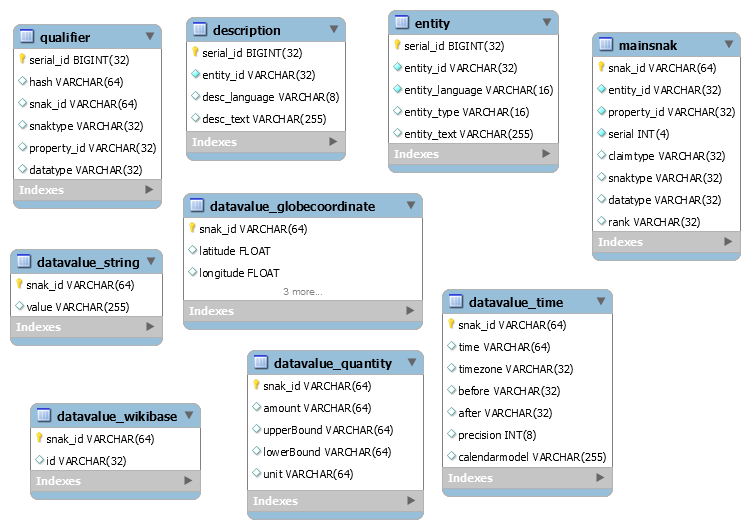
\includegraphics[width=0.8\linewidth]{datadetail.png}
\caption{Details of our table design}
\end{figure*}
\subsection{datavalue\_quantity}
\lstset{language=SQL}
Table schema:
\begin{lstlisting}
CREATE TABLE IF NOT EXISTS `wikidata`.`datavalue_quantity` (
  `snak_id` VARCHAR(64) NOT NULL,
  `amount` VARCHAR(64) NULL DEFAULT NULL,
  `upperBound` VARCHAR(64) NULL DEFAULT NULL,
  `lowerBound` VARCHAR(64) NULL DEFAULT NULL,
  `unit` VARCHAR(64) NULL DEFAULT NULL,
  PRIMARY KEY (`snak_id`))
ENGINE = InnoDB
\end{lstlisting}
The data strored in corresponding fields:
\begin{itemize}
\item \textbf{snak\_id}: Primary key. Refering to the table mainsnak.
\item \textbf{amount}: The nominal value of the quantity, as an arbitrary precision decimal string. The string always starts with a character indicating the sign of the value, either "+" or "-".
\item \textbf{upperBound}: Optionally, the upper bound of the quantity's uncertainty interval, using the same notation as the amount field.
\item \textbf{lowerBound}: Optionally, the lower bound of the quantity's uncertainty interval, using the same notation as the amount field.
\item \textbf{unit}: the URI of a unit (or "1" to indicate a unit-less quantity).
\end{itemize}
\subsection{datavalue\_wikibase}
\lstset{language=SQL}
Table schema:
\begin{lstlisting}
CREATE TABLE IF NOT EXISTS `wikidata`.`datavalue_wikibase` (
  `snak_id` VARCHAR(64) NOT NULL,
  `id` VARCHAR(32) NULL DEFAULT NULL,
  PRIMARY KEY (`snak_id`))
ENGINE = InnoDB
\end{lstlisting}
The data strored in corresponding fields:
\begin{itemize}
\item \textbf{snak\_id}: Primary key. Refering to the table mainsnak.
\item \textbf{id}: defines the id of the entity.
\end{itemize}
\subsection{qualifier}
\lstset{language=SQL}
Table schema:
\begin{lstlisting}
CREATE TABLE IF NOT EXISTS `wikidata`.`qualifier` (
  `serial_id` BIGINT(32) NOT NULL AUTO_INCREMENT,
  `hash` VARCHAR(64) NULL DEFAULT NULL,
  `snak_id` VARCHAR(64) NULL DEFAULT NULL,
  `snaktype` VARCHAR(32) NULL DEFAULT NULL,
  `property_id` VARCHAR(32) NULL DEFAULT NULL,
  `datatype` VARCHAR(32) NULL DEFAULT NULL,
  INDEX `STYPE` (`snaktype` ASC),
  INDEX `PID` (`property_id` ASC),
  INDEX `DTYPE` (`datatype` ASC),
  PRIMARY KEY (`serial_id`),
  INDEX `SID` (`snak_id` ASC),
  INDEX `HASH` (`hash` ASC))
ENGINE = InnoDB
\end{lstlisting}
The data strored in corresponding fields:
\begin{itemize}
\item \textbf{serial\_id}: Primary key.
\item \textbf{hash}: Hash value of qualifier. Used to build connection between table qualifier and datavalue\_ series.
\item \textbf{snak\_id}: The id of the snak this qualifier belongs to. Used to build connection between table qualifier and mainsnak.
\item \textbf{snaktype}: Similar to the table mainsnak.
\item \textbf{property\_id}: Similar to the table mainsnak.
\item \textbf{datatype}: Similar to the table mainsnak.
\end{itemize}
In Figure 2
\section{DATA POPULATING}
Populating the database - Python script:

In order to populate the database, we have written a Python script to read the JSON file line by line and extract the information that we need. The populating process is as follows:

First we extract the entity ID and entity type, followed by the various languages supported, along with their corresponding descriptions. Once we have this information, we are able to populate both the entity and description tables. Using PyMySQL, we can connect to the MySQL database and effectively insert records. This is followed by the iteration of each property within the claims to populate the remaining tables. We extract information from the mainsnak and qualifiers to insert into the mainsnak table and qualifier table respectively.

Then, we deal with the various types of data values that we may encounter in the mainsnaks and qualifiers. This includes string, wikibase-entityid, time, globecoordinate, and quantity types. For each type, we extract the necessary fields needed to populate the corresponding table. We insert these records in the same fashion as before, and continue on to the next iteration.

\section{DATABASE OVERVIEW}

Due to the constraint of disk size, we only use 100k entities as the set for our experiment. The experiment on the next section is based on the subset below.

Overall statistics:
\begin{center}
  \begin{tabular}{ | c | c |}
    \hline
    name & count \\ \hline\hline
    entity & 999999 \\ \hline
    item & 999323 \\ \hline
    property & 676 \\
    \hline
  \end{tabular}
\end{center}

Table statistics:
\begin{center}
  \begin{tabular}{ | c | c |}
    \hline
    table & row number \\ \hline\hline
    datavalue\_globecoordinate & 201934 \\ \hline
    datavalue\_quantity & 204015 \\ \hline
    datavalue\_string & 2759499 \\ \hline
    datavalue\_time & 463418 \\ \hline
    datavalue\_wikibase & 4501342 \\ \hline
    description & 6836149 \\ \hline
    entity & 10430881 \\ \hline
    mainsnak & 7720798 \\ \hline
    qualifier & 2759499 \\
    \hline
  \end{tabular}
\end{center}

\section{QUERY DESIGN}
\subsection{Query 1}
\subsubsection{Design}
\subsubsection{Performance}
Sampling 5 examples:
\begin{center}
  \begin{tabular}{ | c | c | c |}
    \hline
    serial & entity & time \\ \hline\hline
    1 & universe & 0.016sec \\ \hline
    2 & dig & 0.015sec \\ \hline
    3 & flower & 0.016sec \\ \hline
    3 & president & 0.016sec \\ \hline
    3 & like '\%mi\%' & 0.172sec \\
    \hline
  \end{tabular}
\end{center}
\subsection{Query 2}
\subsubsection{Design}
\subsubsection{Performance}
Sampling 5 examples:
\begin{center}
  \begin{tabular}{ | c | c | c |}
    \hline
    serial & entity & time \\ \hline\hline
    1 & universe & 0.047sec \\ \hline
    2 & apple & 0.015sec \\ \hline
    3 & mud & 0.016sec \\ \hline
    3 & fly & 0.032sec \\ \hline
    3 & wind & 0.032sec \\
    \hline
  \end{tabular}
\end{center}
\subsection{Query 3}
\subsubsection{Design}
\subsubsection{Performance}
Sampling 5 examples:
\begin{center}
  \begin{tabular}{ | c | c | c |}
    \hline
    serial & entity & time \\ \hline\hline
    1 & universe & 0.031sec \\ \hline
    2 & car & 0.032sec \\ \hline
    3 & noodle & 0.031sec \\ \hline
    3 & dragon & 0.094sec \\ \hline
    3 & china & 3.171sec \\
    \hline
  \end{tabular}
\end{center}
\subsection{Query 4}
\subsubsection{Design}
\subsubsection{Performance}
Sampling 5 examples:
\begin{center}
  \begin{tabular}{ | c | c | c |}
    \hline
    serial & entity & time \\ \hline\hline
    1 & gas & 0.031sec \\ \hline
    2 & kill & 0.000sec \\ \hline
    3 & fix & 0.000sec \\ \hline
    3 & dare & 0.006sec \\ \hline
    3 & knock & 0.016sec \\
    \hline
  \end{tabular}
\end{center}
\subsection{Extra Queries}
10' bonus.我觉得你就写点有的没的,比如把q2的父亲变儿子之类?
\subsubsection{Given an entity, return all the entities belongs to this entity.}
\section{USER INTERFACE DESIGN}
\subsection{Query interface}
\subsection{Q\&A interface}

\end{document} 
